%% abtex2-modelo-slides.tex, v-1.0 gfabinhomat
%% Copyright 2012-2015 by abnTeX2 group at http://www.abntex.net.br/ 
%%
%% This work may be distributed and/or modified under the
%% conditions of the LaTeX Project Public License, either version 1.3
%% of this license or (at your option) any later version.
%% The latest version of this license is in
%%   http://www.latex-project.org/lppl.txt
%% and version 1.3 or later is part of all distributions of LaTeX
%% version 2005/12/01 or later.
%%
%% This work has the LPPL maintenance status `maintained'.
%% 
%% The Current Maintainer of this work is Fábio Rodrigues Silva, 
%% member of abnTeX2 team, led by Lauro César Araujo. 
%% Further information are available on 
%% http://www.abntex.net.br/
%%
%% This work consists of the files abntex2-modelo-slides.tex, 
%% abntex2-modelo-references.bib and abntex2-modelo-marca.pdf
%%
%% Modelo desenvolvido por Fábio Rodrigues Silva (gfabinhomat@gmail.com)
%% Mais informações podem ser obtidas no guia do usuário Beamer 
%% (http://linorg.usp.br/CTAN/macros/latex/contrib/beamer/doc/beameruserguide.pdf)
%% Informações rápidas podem ser acessadas em http://en.wikibooks.org/wiki/LaTeX/Presentations


% Apresentações em widescreen. Outros valores possíveis: 1610, 149, 54, 43 e 32.
% Por padrão, as apresentações são no formato 4:3 (sem o aspectratio).
\documentclass[aspectratio=169]{beamer}	 	

\usetheme{Berlin}
\usecolortheme{dolphin}
\usefonttheme[onlymath]{serif}			% para fontes matemáticas
% Enconte mais temas e cores em http://www.hartwork.org/beamer-theme-matrix/ 
% Veja também http://deic.uab.es/~iblanes/beamer_gallery/index.html

% Customizações de Cores: fg significa cor do texto e bg é cor do fundo
% ---
% PACOTES
% ---
\usepackage[alf]{abntex2cite}		% Citações padrão ABNT
\usepackage[brazil]{babel}		% Idioma do documento
\usepackage{color}			% Controle das cores
\usepackage[T1]{fontenc}		% Selecao de codigos de fonte.
\usepackage{graphicx}			% Inclusão de gráficos
\usepackage[utf8]{inputenc}		% Codificacao do documento (conversão automática dos acentos)
\usepackage{txfonts}			% Fontes virtuais
\usepackage{ragged2e}
% ---
\usepackage{caption}
% --- Informações do documento ---
\title{Comparação entre o método dos Mínimos Quadrados e Maximização da Correntropia do Erro aplicados ao Controle Adaptativo}

\author{Allan de Medeiros Martins \\
        Pedro Yochinori Gushiken}
\institute{Universidade Federal do Rio Grande do Norte}
\date{06 de dezembro de 2016}
% ---

% ----------------- INÍCIO DO DOCUMENTO --------------------------------------
\begin{document}

% ----------------- NOVO SLIDE --------------------------------
\begin{frame}

\begin{minipage}{1\linewidth}
  \centering
\end{minipage}

\titlepage

\end{frame}

% ----------------- NOVO SLIDE --------------------------------
\begin{frame}{Sumário}
\tableofcontents
\end{frame}

% ----------------- NOVO SLIDE --------------------------------
\section{Introdução}
\begin{frame}
\frametitle{Contextualização}
\begin{enumerate}
\item<1-> Controle por Posicionamento de Polos\\
\item<2-> Estimação, Caso Indireto\\ 
\item<3-> Correntropia e Controle\\
\end{enumerate}
\end{frame}


% ----------------- NOVO SLIDE --------------------------------
\section{Conceitos}
\subsection{Parametrização}

\begin{frame}
\frametitle{Descrições}
Seja a planta controlável e observável descrita por sua função de transferência:
\begin{equation*}
G_p(s) = \frac{N_p(s)}{D_p(s)} = \frac{b_0 + b_1 s + ... + b_{n-1} s^{n-1}}{a_0 + a_1 s+ ... + a_n s^n}
\end{equation*}

Onde apenas os sinais $u(t) \in R^1$ e $y(t) \in R^1$ estão disponíveis para medição.
\end{frame}

\begin{frame}
Uma parametrização alternativa da planta é da seguinte forma:

\begin{equation*}
\theta^* = [b_{n-1}, b_{n-2}, ...~ , b_1, b_0, a_{n-1}, a_{n-2}, ...~ , a_1, a_0]^T
\end{equation*}

\begin{equation*}
Y = [u^{(n-1)},u^{(n-2)},...,u,-y^{(n-1)},-y^{(n-2)},-y]
\end{equation*}


\begin{equation*}
y = {\theta^*}^T Y
\end{equation*}


\end{frame}


\begin{frame}

Seja um polinômio $\Lambda(s)$ cujas raízes tem todas parte real negativa:
\begin{equation*}
\Lambda(s) = s^n + \lambda_{n-1} s^{n-1} + ... + \lambda_0
\end{equation*}

E um vetor $\alpha_{n-1}(s)$:

\begin{equation*}
\alpha_{n-1} = [s^{(n-1)},s^{(n-2)},...,s^0]^T
\end{equation*}

\end{frame}

\begin{frame}

Desejamos estimar os $2n$ parâmetros da planta, mas dispomos de apenas 2 sinais. De tal forma que criamos um regressor a partir de $u(t)$ e $y(t)$ e de um filtro estável com polinômio $\Lambda(s)$ no denominador:

\begin{equation*}
\phi_1 = \frac{\alpha_{n-1}(s)}{\Lambda(s)} u
\end{equation*}

\begin{equation*}
\phi_2 = -\frac{\alpha_{n-1}(s)}{\Lambda(s)} y
\end{equation*}

E criamos um regressor $\phi(t)$ concatenando $\phi_1(t)$ e $\phi_2(t)$.
\end{frame}


\begin{frame}

Passando $y(t)$ pelo filtro com $\Lambda(s)$ no denominador criamos um novo sinal $z(t)$:

\begin{equation*}
z = \frac{s^n y}{\Lambda(s)}
\end{equation*}

É válida a seguinte parametrização de $z(t)$:

\begin{equation*}
z = {\theta^*}^T \phi
\end{equation*}


\end{frame}

\begin{frame}
Caracterizamos então uma estimativa de $z(t)$ da seguinte forma:

\begin{equation*}
\hat{z} = \theta^T \phi
\end{equation*}

E o erro normalizado entre estes sinais:

\begin{equation*}
\epsilon = \frac{z - \hat{z}}{m^2}
\end{equation*}

Onde $m = 1+n_s^2$ tal que $\phi/m \in \mathcal{L}_\infty$. [escolhas comum: $n_s^2 = \phi^T\phi$]

\end{frame}

\subsection{Estimação dos Parâmetros da Planta usando LSE}
\begin{frame}
Para o algoritmo "Least Square Error"(LSE) recursivo com fator de esquecimento, escolhemos a seguinte função de custo com fator de esquecimento:

\begin{equation*}
 J(\theta) = \frac{1}{2} \int_{0}^{t} e^{-\beta(t - \tau)} \frac{[z(\tau) - \theta^T(t)\phi(\tau)]}{m^2(\tau)} d\tau
        + \frac{1}{2} e^{-\beta t}(\theta - \theta_0)^TQ_0(\theta - \theta_0)
\end{equation*}

\end{frame}

\begin{frame}
Esta função de custo leva ao gradiente:
\begin{equation*}
\nabla J(\theta) = e^{-\beta t}Q_0 (\theta(t)-\theta_0)
                    -\int_{0}^t e^{-\beta(t - \tau)} \frac{[z(\tau) - \theta^T(t)\phi(\tau)]}{m^2(\tau)}\phi(\tau) d\tau
\end{equation*}

Que leva à seguinte implementação de uma lei de atualização para as estimativas $\theta$:

\begin{equation*}
\begin{array}{l}
\dot{P} = \beta P - P\frac{\phi \phi^T}{m^2}P\\
\dot{\theta} = P\epsilon \phi
\end{array}
\end{equation*}

\end{frame}

\subsection{Estimação dos Parâmetros da Planta usando critério de maximização da Correntropia}
\begin{frame}
Seja um estimador da correntropia entre as variáveis aleatórias $Z$ e $\hat{Z}$ avaliado a partir de uma única amostra:

\begin{equation*}
\hat{V}(Z,\hat{Z}) =\frac{1}{\sqrt{2\pi}\sigma} e^{-(z_i - \hat{z}_i)^2/2\sigma^2}
\end{equation*}

Escolhemos este estimador como função de custo:

\begin{equation*}
\hat{V}(Z,\hat{Z}) = J(\theta)
\end{equation*}

E esperamos que $\hat{V}(Z,\hat{Z})$ tenha um comportamento similar ao valor esperado $V(Z,\hat{Z}) = \mathbf{E}(k_\sigma(Z-\hat{Z}))$ que é a correntropia exata. Este raciocínio é similar ao aplicado em alguns algoritmos de gradiente estocástico.

\end{frame}

\begin{frame}
Somos então levados ao gradiente:

\begin{equation*}
\nabla J(\theta) = \epsilon \phi \frac{1}{\sqrt{2\pi}\sigma^3} e^{-\frac{\epsilon^2}{2 \sigma^2}}  
\end{equation*}

E uma escolha possível para a lei de atualização dos parâmetros $\theta$ é:

\begin{equation*}
\dot{\theta} = \Gamma \nabla J(\theta)
\end{equation*}

Com  $\Gamma \in \mathcal{R}^{2n\times2n}$, $\Gamma = \Gamma^T > 0$.
\end{frame}

\begin{frame}
Assim, fazendo uso do conceito de correntropia somos levados ao estimador:
\begin{equation*}
\dot{\theta} = \Gamma \epsilon \phi \frac{1}{\sqrt{2\pi}\sigma^3} e^{-\frac{\epsilon^2}{2\sigma^2}}
\end{equation*}

E podemos estimar os parâmetros da planta em tempo real fazendo uso do conceito de correntropia.

\end{frame}



\subsection{Controle por Posicionamento de Polos}
\begin{frame}
Seja um controlador usando o princípio do modelo interno, tal que $Q_m(s)$ cancele os termos instáveis dos sinais de referência e perturbação:
\begin{equation*}
C(s) = \frac{P(s)}{L(s)Q_m(s)}
\end{equation*}

E lembrando que:
\begin{equation*}
G_p(s) = \frac{N_p(s)}{D_p(s)}
\end{equation*}

\end{frame}

\begin{frame}
\frametitle{Descrições, Cont.}

Em realimentação unitária, o polinômio no denominador da função de transferência em malha fechada é:

\begin{equation*}
L(s)Q_m(s)D_p(s) + N_p(s)P(s) = A^*(s)
\end{equation*}

Ou seja, resolvendo para $L(s)$ e $P(s)$ podemos obter um polinômio desejado $A^*(s)$ em malha fechada, desde que conheçamos $D_p(s)$ e $N_p(s)$.\\

No controle adaptativo substituímos os parâmetros da planta contidos em $D_p(s)$ e $N_p(s)$ desconhecidos por suas estimativas.

\end{frame}

\begin{frame}
\frametitle{Equações, Cont.}

De tal forma que a seguinte lei de controle é gerada:

\begin{equation*}
u_p = (\Lambda - \hat{L} Q_m)\frac{1}{\Lambda} u_p - \hat{P} \frac{1}{\Lambda}(y_p - r)
\end{equation*}

Onde $r$ é uma referência qualquer escolhida. 

\end{frame}


% ----------------- NOVO SLIDE --------------------------------
\section{Simulações}
% % % % % % % % % % % % % % % % % % % % % % % % % % % % % % % % % % %
\subsection{APPC}
\begin{frame}
\centering
  \begin{minipage}{.48\textwidth}
  	\begin{figure}
  	 \centering
     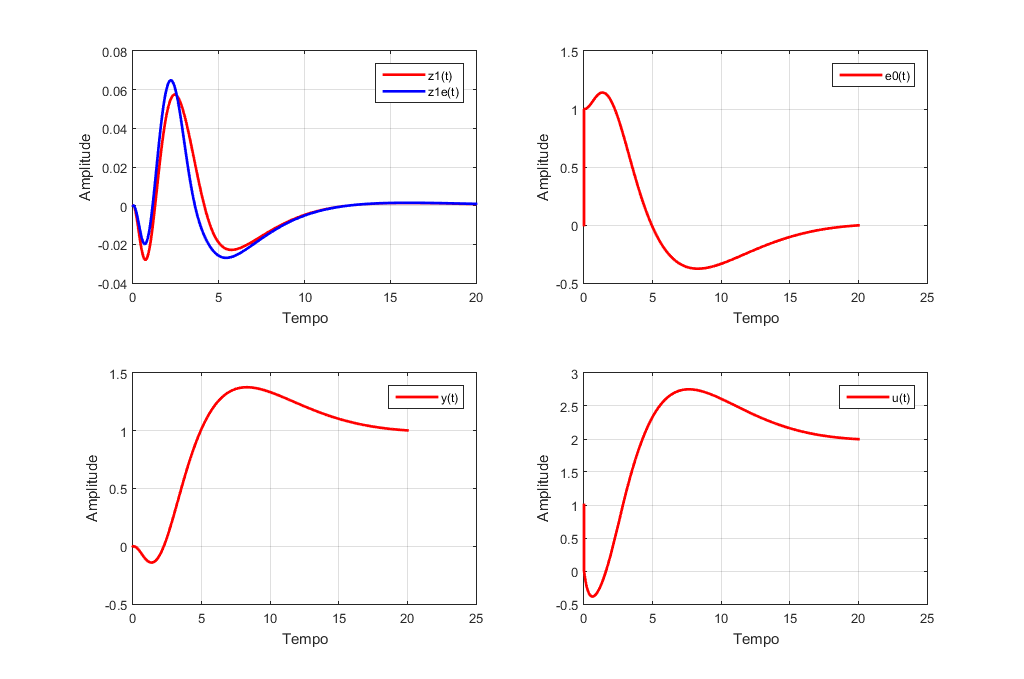
\includegraphics[width=0.8\linewidth]{./pics/APPC_Correntropia_Ideal.png}
     \caption{Comportamento do controlador Adaptativo por Posicionamento de Polos(APPC) em um ambiente sem ruído com estimador por Maximização da Correntropia do Erro}
  	\end{figure}
  \end{minipage}
  \hfill
  \begin{minipage}{.48\textwidth}
  	\begin{figure}
  	 \centering
     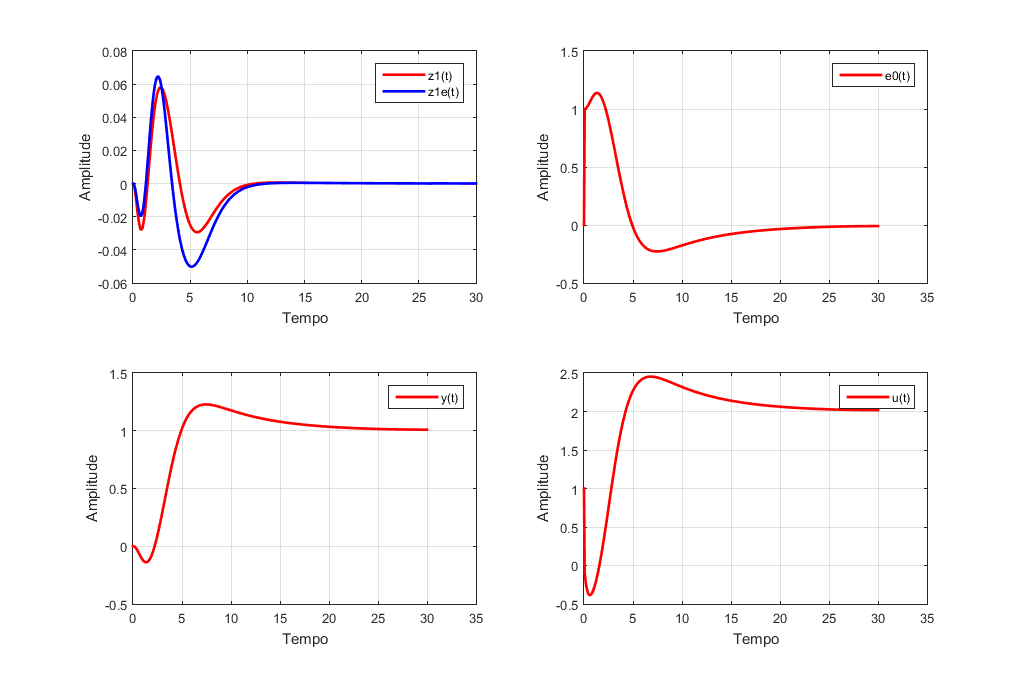
\includegraphics[width=0.8\linewidth]{./pics/APPC_MSE_Ideal.png}
     \caption{Comportamento do controlador Adaptativo por Posicionamento de Polos(APPC) em um ambiente sem ruído com estimador por Minimização do Erro Quadrado com Fator de Esquecimento}
  	\end{figure}
  \end{minipage}
\end{frame}

\begin{frame}
\centering
  \begin{minipage}{.48\textwidth}
  	\begin{figure}
  	 \centering
     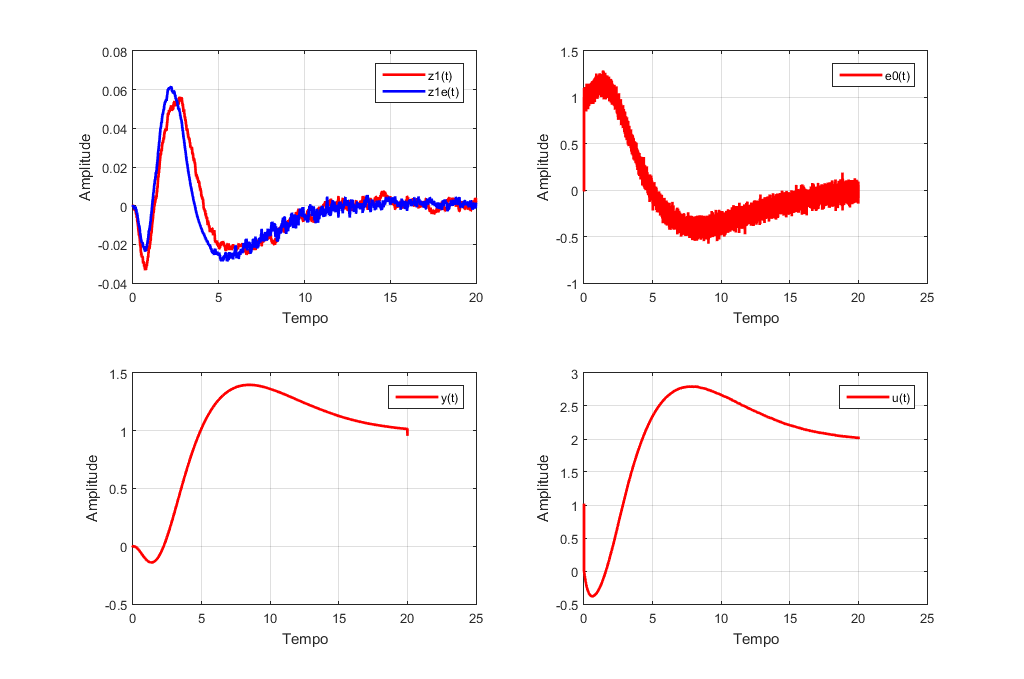
\includegraphics[width=0.8\linewidth]{./pics/APPC_Correntropia_Ruido_Gaussiano.png}
     \caption{APPC-MCC em ambiente com ruído gaussiano}
  	\end{figure}
  \end{minipage}
  \hfill
  \begin{minipage}{.48\textwidth}
  	\begin{figure}
  	 \centering
     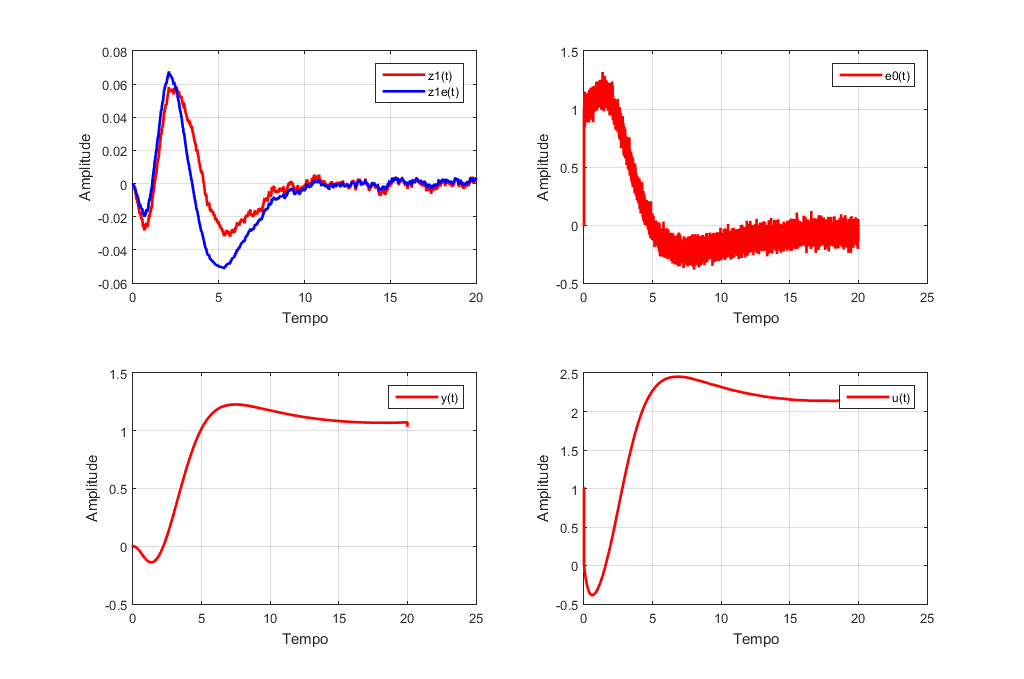
\includegraphics[width=0.8\linewidth]{./pics/APPC_MSE_Ruido_Gaussiano.png}
     \caption{APPC-LSE em ambiente com ruído gaussiano}
  	\end{figure}
  \end{minipage}
\end{frame}
\begin{frame}
\centering
  \begin{minipage}{.48\textwidth}
  	\begin{figure}
  	 \centering
     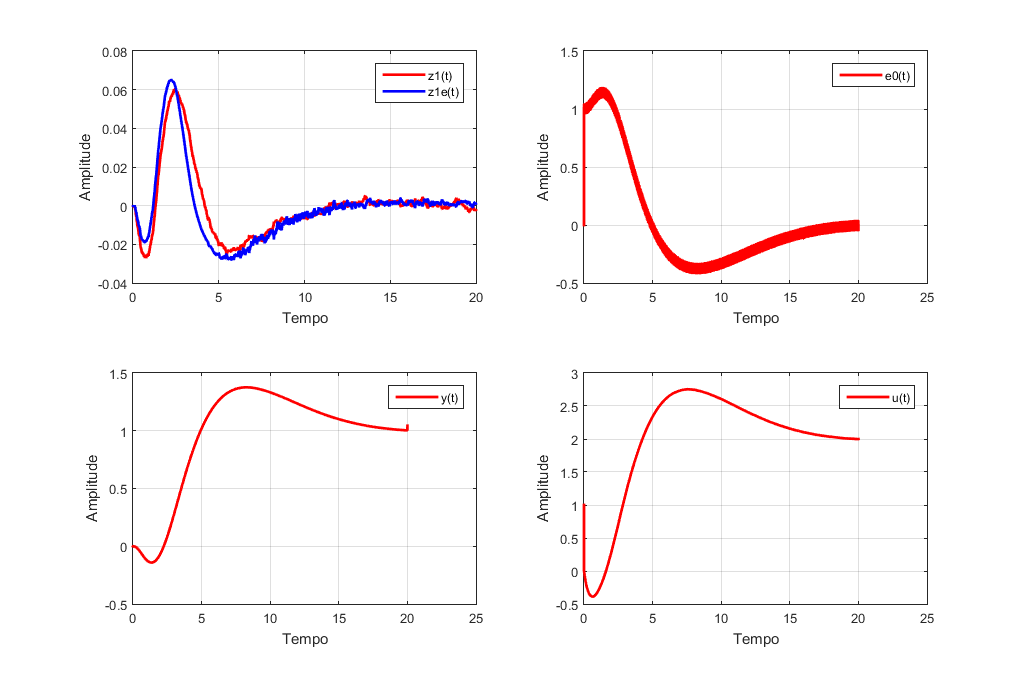
\includegraphics[width=0.8\linewidth]{./pics/APPC_Correntropia_Ruido_Uniforme.png}
     \caption{APPC-MCC em ambiente com ruído uniforme}
  	\end{figure}
  \end{minipage}
  \hfill
  \begin{minipage}{.48\textwidth}
  	\begin{figure}
  	 \centering
     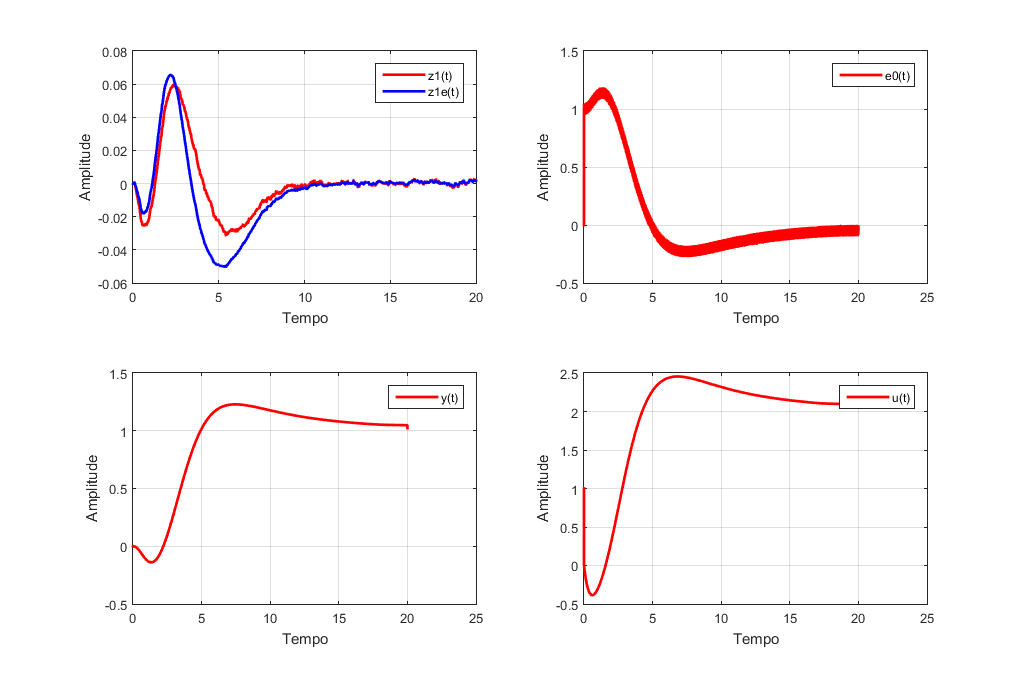
\includegraphics[width=0.8\linewidth]{./pics/APPC_MSE_Ruido_Uniforme.png}
     \caption{APPC-LSE em ambiente com ruído uniforme}
  	\end{figure}
  \end{minipage}
\end{frame}


\begin{frame}
\centering
  \begin{minipage}{.48\textwidth}
  	\begin{figure}
  	 \centering
     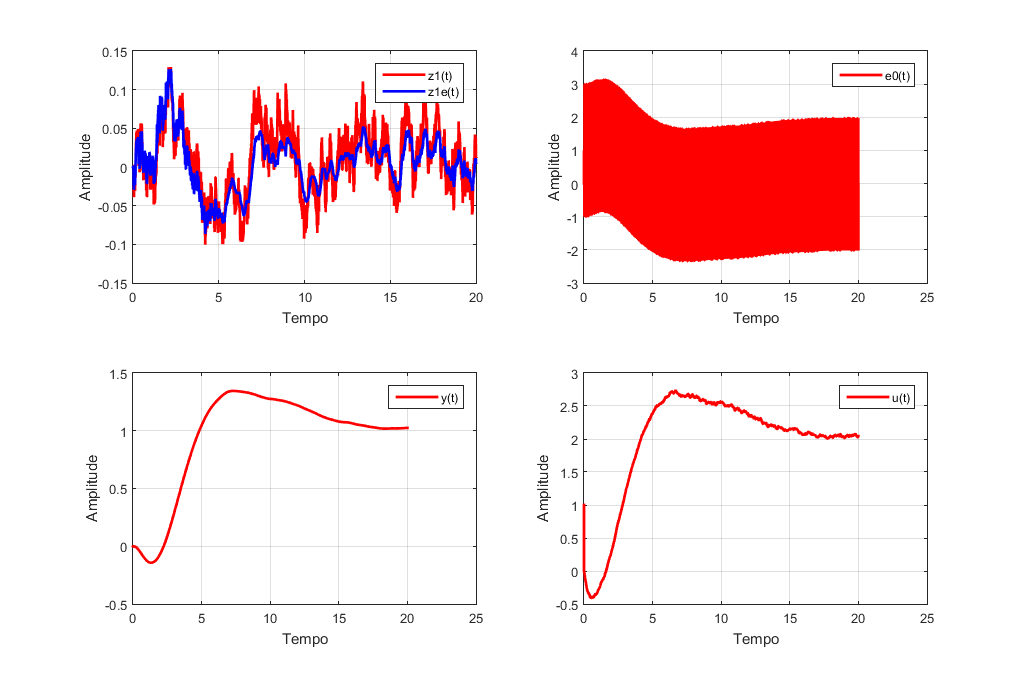
\includegraphics[width=0.8\linewidth]{./pics/APPC_Correntropia_Ruido_Impulsivo.png}
     \caption{APPC-MCC em ambiente com ruído impulsivo, falha do controlador, instabilidade}
  	\end{figure}
  \end{minipage}
  \hfill
  \begin{minipage}{.48\textwidth}
  	\begin{figure}
  	 \centering
     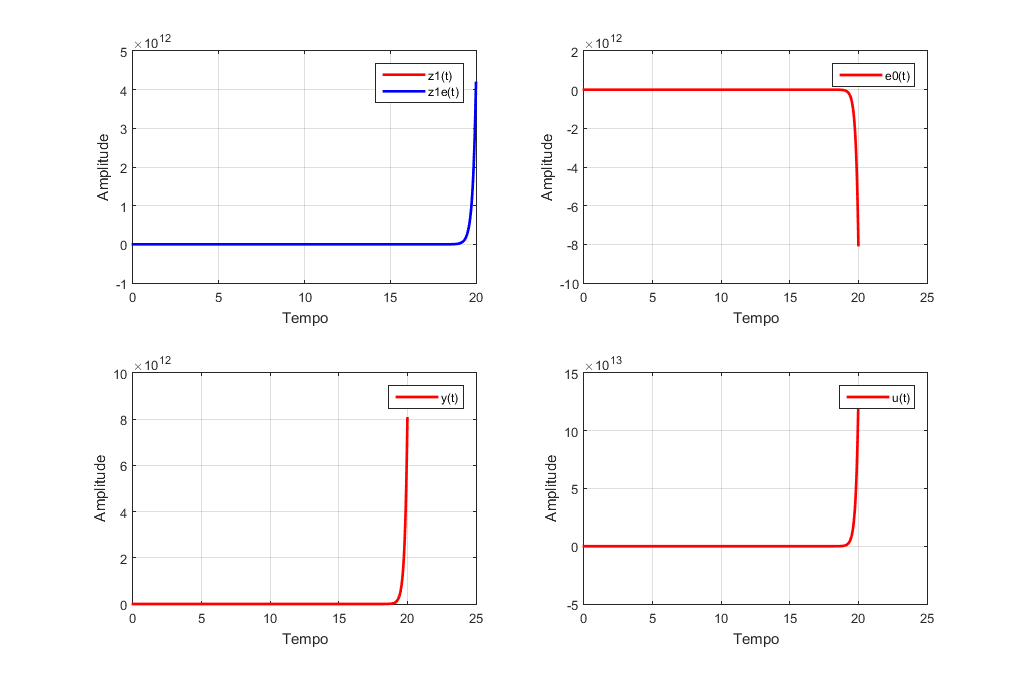
\includegraphics[width=0.8\linewidth]{./pics/APPC_MSE_Ruido_Impulsivo.png}
     \caption{APPC-LSE em ambiente com ruído impulsivo}
  	\end{figure}
  \end{minipage}
\end{frame}

% ----------------- NOVO SLIDE --------------------------------
\section{Conclusão}
\begin{frame}
\frametitle{Conclusão}

A Maximização da Correntropia do erro como critério de estimação de parâmetros discutida para este artigo apresenta:

\begin{itemize}
\item[1] Desempenho comparável ao LSE quando aplicada ao controle
\item[2] Capacidade de rejeição do ruído impulsivo
\item[3] Compatibilidade com estratégias de Controle Indireto
\end{itemize}

Em trabalhos futuros trataremos de uma fundamentação matemática mais robusta e condições suficientes de convergência das estimativas para o algoritmo proposto. Muito obrigado!

\end{frame}


% --- O comando \allowframebreaks ---
% Se o conteúdo não se encaixa em um quadro, a opção allowframebreaks instrui 
% beamer para quebrá-lo automaticamente entre dois ou mais quadros,
% mantendo o frametitle do primeiro quadro (dado como argumento) e acrescentando 
% um número romano ou algo parecido na continuação.
% --- O comando \allowframebreaks ---
% Se o conteúdo não se encaixa em um quadro, a opção allowframebreaks instrui 
% beamer para quebrá-lo automaticamente entre dois ou mais quadros,
% mantendo o frametitle do primeiro quadro (dado como argumento) e acrescentando 
% um número romano ou algo parecido na continuação.

%\begin{frame}
%\frametitle{Referências}
%\nocite{narendra1}
%\nocite{narendra_main}
%\nocite{narendra2012rationale}
%\nocite{narendra1997}
%\nocite{han1}
%\nocite{han2010}
%\nocite{han2012}
%\nocite{kuipers1}
%\nocite{ioannou2}
%\nocite{chen}
%nocite{ogata}
% %nocite{khalil}
%\end{frame}
\nocite{Bottou2010,chen2,chen,principebook,principe1,ogata,ioannou2, tao,krstic}
% ----------------- FIM DO DOCUMENTO -----------------------------------------
\bibliography{bib-controleadaptativo}
\end{document}
